\ylDisplay{Propeller} % Ülesande nimi
{Andreas Valdmann} % Autor
{lõppvoor} % Voor
{2010} % Aasta
{G 10} % Ülesande nr.
{10} % Raskustase
{
% Teema: Kinemaatika
\ifStatement
See pilt pöörlevast lennukipropellerist on tehtud telefoni kaameraga, mis salvestab korraga ühe vertikaalse veeru pikselid. Pilt tekib vasakult paremale veergude kaupa skaneerides.\\
\osa Mis suunas pöörleb propeller fotograafi poolt vaadatuna (päripäeva või vastupäeva)?\\
\osa Mitu laba on propelleril?\\
\osa Mitu pööret teeb propeller ühes minutis, kui kogu pildi tegemiseks kulunud aeg on 1/8 sekundit?\\

\begin{center}
	\includegraphics[width=90mm]{2010-v3g-10-Propeller.jpg}
\end{center}
\fi


\ifHint
\osa
Vastavalt sellele kas labad liiguvad salvestatavatele pikselite veergudele vastu või eemale, on labade kujutiste tihedus vastavalt suurem või väiksem.\\
\osa
Vaadeldes pildil ühte vertikaalset pikselite veergu ei ole moonutusi näha. Seega tasub uurida kui palju labasid erinevatel pikselite veergudel näha on.\\
\osa
Teades labade arvu on võimalik vaadelda täpselt kui palju üks laba salvestamise käigus liigub.
\fi


\ifSolution
\osa Propeller pöörleb vastupäeva, sest pildi ülaosas liiguvad labad vastu parajasti salvestatavale pikseliveerule ja seetõttu paiknevad seal labade kujutised tihedamalt.\\
\osa Vasakpoolsesl joonisel on ülalt alla tõmmatud üks veerg millel on korraga peal maksimaalset 2 laba. Kui labasid oleks 2, peaks veerus paistma korraga vaid üks laba. Labad ise on kantud joonisele mustaga. Näha on, et labade vaheline nurk on suurem kui 90 kraadi ja seega propeller on 3-labaline.

\begin{center}
	\includegraphics[width=50mm]{2010-v3g-10-Propeller2.jpg}
	\qquad
	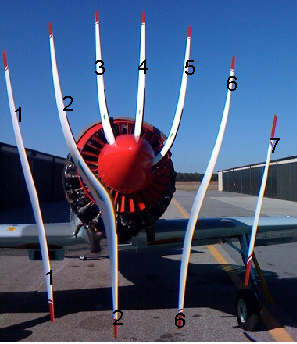
\includegraphics{2010-v3g-10-proplah}
\end{center}

\textit{Alternatiivne lahendus} \\
Tähistame labade tekitatud jooned numbritega 1 kuni 7 nii nagu näidatud parempoolsel joonisel.
Joonise alumises servas eelneb joon 2 joonele 6.
See tähendab, et joonele 2 vastav laba peab eelnema joonele 6 vastavale labale.
Joonise ülemise serva põhjal võime analoogselt väita, et joonele 5 vastav laba peab eelnema joonele 6 vastavale labale.
Järelikult peavad jooned 5 ja 2 vastama samale labale. Ülemises servas jääb joonte 5 ja 2 vahele veel 2
joont, st sellele labale vastavad jooned korduvad perioodiga 3 joont.
See periood peab olema propelleri labade arvu $n$ kordne. Et 3 on algarv, siis ainus variant on $n=3$.\\
\osa Iga kolmas triip pildil kujutab sama propellerilaba. Järgneval joonisel on valgega nummerdatud labad;
propelleri telje kõrgusel on tõmmatud joon mille kogupikkus moodustus pildistamise aja jooksul ehk kogupikkus on $1/8\;$s.
Punasega on märgitud aeg millega laba number üks jõudis liikuda 1,5 pööret. (joonisel mustaga)
Punase osa pikkus moodustab ligikaudu 4/5 pildi kogulaiusest. Seetõttu moodustab ka nende punktide ajaline intervall 4/5 pildi tegemise koguajast. Selle aja jooksul teeb propeller poolteist pööret. Ühes sekundis teeb propeller $\num{1,5} /(1/8\cdot 4/5)=15$ pööret ja ühes minutis $15\cdot 60=900$ pööret.

\begin{center}
	\includegraphics[width=50mm]{2010-v3g-10-Propeller3.jpg}
\end{center}
\fi
}